\chapter{압력, 자유 에너지, 에너지 요동}

\lectureoverview{분자가 벽에 부딪히는 운동론적 그림을 가정하지 않고 분배함수로부터 압력을 유도한다. 기하학적 보조정리를 이용해 단열 미분을 고정 온도 미분으로 바꾸고, 헬름홀츠 자유 에너지로 \(\log Z\)와 연결한 뒤 첫 적용 사례로 이상기체 법칙을 얻는다. 이어 같은 분배함수를 사용해 평형 에너지 요동과 열용량의 관계를 유도한다.}

\section{수학으로 직관을 검증하기}

열역학에는 묘한 평판이 따라다닌다. 미적분 자체는 기초적이지만, 무엇을 미분하고 무엇을 고정할지를 정하는 일은 놀라울 만큼 까다로울 수 있다. 여기서 다룰 문제의 범위는 의도적으로 좁다. 이상기체의 압력을 계산하는 것이다. 그러나 답을 구하는 과정은 익숙한 분자 그림이 더는 믿을 만하지 않은 계에도 충분히 일반적으로 적용되도록 구성한다.

운동론적 설명은 간단하다. 분자가 벽에 부딪혀 운동량의 법선 성분을 반전시킨다. 단위 시간당 전달되는 운동량이 힘을 주고, 단위 면적당 힘이 압력을 준다. 이미 3차원에서 분자 하나의 평균 운동 에너지가 다음과 같음을 알고 있다.
\begin{equation}
 \left\langle \frac{p^2}{2m}\right\rangle=\frac{3}{2}T
 \qquad (k_B=1).
 \label{eq:sm5-mean-kinetic-energy}
\end{equation}
속도 분포가 등방적이면 충돌률과 충돌마다 전달되는 운동량, 그리고 그 결과 생기는 압력을 추산할 수 있다.

하지만 벽이 있으면 등방성이 깨지는 듯하다. 경계 바로 근처의 분자들이 내부 깊숙한 곳의 분자들과 같은 속력 및 방향 분포를 가진다고 어떻게 확신할 수 있을까? 평형 상태에서는 여기서 필요한 정확도 범위 내에서 실제로 그렇다. 그러나 그 결론은 직관으로 계산에 몰래 끼워 넣을 것이 아니라 통계역학에서 따라 나와야 한다. 분자들끼리 충돌하면 운동론적 논증은 더욱 불투명해진다. 비상호작용 기체가 다루기 쉬운 것은 바로 그것이 유난히 단순한 계이기 때문이다.

물리학에는 그림을 잠시 접어 두고 수학을 따라가는 것이 가장 안전한 절차인 때가 있다. 구하려는 물리량을 정하고 일반적인 관계식을 변형하다 보면 익숙한 공식이 나타난다. 마지막에 직관이 돌아오지만, 그때는 수학이 직관의 검증자가 되어 있다. 그 반대가 아니다. 이런 과정을 통해 뜻밖의 관계가 드러나는 데 열역학의 묘미가 있다.

구하려는 관계는 상태방정식이다.
\begin{equation}
 P=P(T,V,N),
 \label{eq:sm5-equation-of-state-target}
\end{equation}
여기서 \(N\)는 물질의 양, \(T\)은 온도, \(V\)은 부피다. 입자들이 상호작용하거나 물질이 액체, 플라스마 또는 고체인 경우에도 타당한 유도가 되어야 한다. 분배함수를 마지막으로 계산하는 단계에서만 이상기체라는 특수한 경우를 다룬다.

\section{엔트로피와 헬름홀츠 자유 에너지}

먼저 뒤에서 사용할 정준 앙상블 공식을 되짚어 보자. \(i\)로 표시한 미시상태에 대해,
\begin{equation}
 \begin{aligned}
 S&=-\sum_i p_i\log p_i,\\
 p_i&=\frac{e^{-\beta E_i}}{Z},\\
 Z&=\sum_i e^{-\beta E_i}.
 \end{aligned}
 \label{eq:sm5-canonical-definitions}
\end{equation}
확률의 로그는 다음과 같다.
\begin{equation}
 \log p_i=-\beta E_i-\log Z.
 \label{eq:sm5-log-probability}
\end{equation}
이를 엔트로피 식에 대입하면 다음을 얻는다.
\begin{align}
 S
 &=-\sum_i p_i\log p_i \notag\\
 &=\beta\sum_i p_iE_i+\log Z\sum_i p_i \notag\\
 &=\beta E+\log Z.
 \label{eq:sm5-entropy-log-z}
\end{align}
여기서 \(E=\sum_i p_iE_i\)는 평균 에너지다.

\begin{classroomqa}\audiencequestion{두 번째 항은 왜 상태 수에 \(\log Z\)를 곱한 값이 아니라 \(\log Z\)만 주나요?}
\lecturerresponse{합의 계수는 \(p_i\)이지 \(1\)이 아닙니다. 정규화로 \(\sum_i p_i=1\)을 얻습니다. 같은 말로, 분자에 있는 \(\sum_i e^{-\beta E_i}=Z\)가 분모의 \(Z\)와 약분됩니다. 이 단계에서는 상태 수가 전혀 등장하지 않습니다.
\lecturetimestamp{00:14:25--00:14:55}}\end{classroomqa}

강의 대부분에서 사용하는 에너지 단위에서는
\(\beta=1/T\)입니다. \eqref{eq:sm5-entropy-log-z}에 \(T\)를 곱하고 식을 정리하면 다음을 얻는다.
\begin{equation}
 E-TS=-T\log Z.
 \label{eq:sm5-helmholtz-identity}
\end{equation}
왼쪽의 이 조합은 매우 자주 등장하므로 이름을 붙일 만하다.
\begin{equation}
 A\equiv E-TS,
 \qquad
 A=-T\log Z.
 \label{eq:sm5-helmholtz-definition}
\end{equation}
이것이 헬름홀츠 자유 에너지다. 지금은 그 이름보다 항등식 자체가 중요하다. 압력을 분배함수의 미분으로 바꿀 때 이 항등식이 필요하다.

\begin{figure}[t]\centering
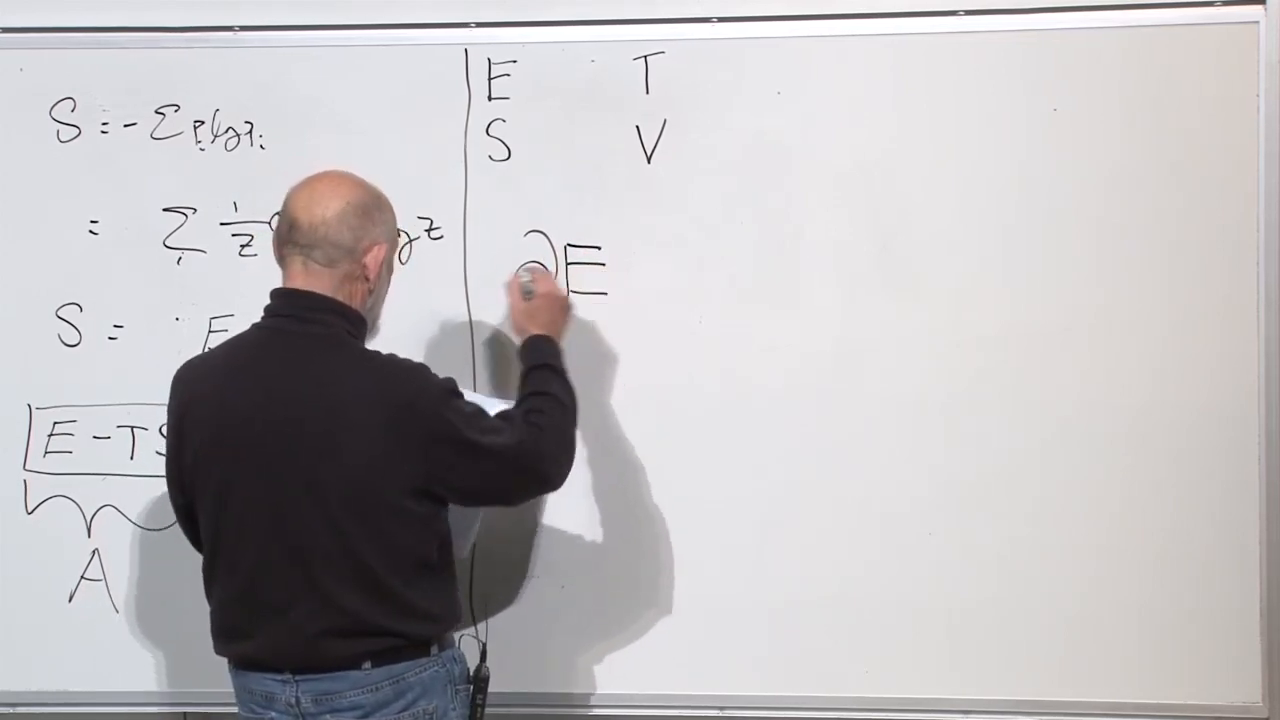
\includegraphics[width=0.90\textwidth]{lecture_05_figure_03.png}\caption{\(A=E-TS=-T\log Z\)}\lectureframe{00:16:50}\end{figure}

\section{제어변수와 그에 대한 응답}

제어변수란 실험자가 외부에서 바꿀 수 있는 거시적 물리량이다. 피스톤을 움직이면 분자 하나하나를 조작하지 않고도 부피를 바꿀 수 있다. 전기장과 자기장을 가하는 것도 다른 예다. 더 일반적인 앙상블에서는 입자 수도 변할 수 있게 둘 수 있다.

열역학 변수는 자연스럽게 켤레쌍을 이룬다. 여기서 부피는 제어변수이고 압력은 그에 대한 응답이다. \(V\)를 바꾸면 압력은 계가 그 변화에 대해 에너지적으로 어떻게 저항하는지 나타낸다. 뒤에서 에너지의 미분을 통해 이 짝 관계를 명확히 하겠다.

\begin{classroomqa}\audiencequestion{압력 자체를 제어변수로 볼 수 있나요?}
\lecturerresponse{외부 압력을 고정하는 실험을 설계할 수도 있습니다. 하지만 여기서 사용하는 구성에서는 피스톤 위치가 부피를 정하고 내부 압력이 응답으로 나타납니다. 압력과 부피는 켤레변수이며, 어느 쪽을 제어하는지는 앙상블과 장치에 따라 달라집니다.
\lecturetimestamp{00:19:22--00:20:01}}\end{classroomqa}

\begin{classroomqa}\audiencequestion{모든 분자가 동일하다고 가정하나요? 아니면 기체에만 적용되는 논증인가요?}
\lecturerresponse{열역학적 논증에는 그런 제한이 필요하지 않습니다. 실린더에는 여러 종의 입자, 액체, 심지어 압축 중인 고체도 담길 수 있습니다. 일반적인 압력 공식을 세운 뒤에야 이상기체 분배함수를 특수한 적용 사례로 다룹니다.
\lecturetimestamp{00:20:02--00:20:39}}\end{classroomqa}

\begin{classroomqa}\audiencequestion{외부에서 조작해 물질의 양을 바꿀 수도 있나요?}
\lecturerresponse{그렇습니다. 입자 수도 가능한 제어변수입니다. 이를 동적으로 다루면 그에 대응하는 켤레변수인 화학 퍼텐셜이 생깁니다. 오늘 계산에서는 \(N\)를 고정해 둡니다.
\lecturetimestamp{00:20:39--00:20:57}}\end{classroomqa}

\begin{classroomqa}\audiencequestion{액체 물과 수증기가 평형 상태에서 동시에 존재할 수 있나요?}
\lecturerresponse{공존 온도와 압력에서는 가능합니다. 중력 때문에 액체가 증기 아래에 놓여도 두 상은 같은 온도를 유지하며 열평형을 이룰 수 있습니다. 여기에도 같은 일반적인 통계역학 체계를 적용할 수 있습니다.
\lecturetimestamp{00:20:59--00:21:36}}\end{classroomqa}

다음 논증에서는 에너지와 엔트로피를 서로 독립적으로 조절할 수 있는 두 변수의 함수로 보자.
\begin{equation}
 E=E(T,V),
 \qquad
 S=S(T,V).
 \label{eq:sm5-dependent-functions}
\end{equation}
온도와 부피는 열역학적 상태 공간의 좌표다. 에너지와 엔트로피는 그 공간의 각 평형점에 값을 부여한다.

\section{엔트로피를 일정하게 유지하는 미분}

궁극적으로 필요한 미분은 특이하다.
\[
 \left(\frac{\partial E}{\partial V}\right)_S.
\]
\(T\)와 \(V\)가 독립 좌표이지만, 이 미분은 종속 함수 \(S(T,V)\)를 일정하게 유지하면서 \(V\)를 변화시키는 경우를 묻는다. 좌표축을 따라가는 미분이 아니라 \((T,V)\) 평면에서 곡선을 따라가는 미분이다.

\begin{classroomqa}\audiencequestion{\(T\)와 \(V\)가 독립인데 나중에 \(dT/dV\)를 어떻게 사용할 수 있나요?}
\lecturerresponse{전체 상태 공간에서는 두 변수가 독립입니다. \(S(T,V)=\mathrm{constant}\)라는 제약을 부과하면 허용되는 상태가 1차원 등고선 위에 놓입니다. 그 등고선을 따라서는 \(V\)의 함수로 \(T\)가 정해지고, 그 기울기 \(dT/dV\)가 정의됩니다.
\lecturetimestamp{01:01:18--01:02:09}}\end{classroomqa}

\begin{lemma}\(E(T,V)\)와 \(S(T,V)\)가 미분 가능하고 \((\partial S/\partial T)_V\neq0\)인 모든 점에서,
\begin{equation}
 \left(\frac{\partial E}{\partial V}\right)_S
 =
 \left(\frac{\partial E}{\partial V}\right)_T
 -
 \left(\frac{\partial E}{\partial S}\right)_V
 \left(\frac{\partial S}{\partial V}\right)_T.
 \label{eq:sm5-calculus-lemma}
\end{equation}\end{lemma}

\begin{proof}임의의 무한소 변위에 대해,
\begin{equation}
 dE=
 \left(\frac{\partial E}{\partial V}\right)_T dV
 +
 \left(\frac{\partial E}{\partial T}\right)_V dT.
 \label{eq:sm5-total-differential-e}
\end{equation}
\(V\)를 고정하면 연쇄법칙에 따라 \(S\)를 중간 변수로 사용할 수 있다.
\begin{equation}
 \left(\frac{\partial E}{\partial T}\right)_V
 =
 \left(\frac{\partial E}{\partial S}\right)_V
 \left(\frac{\partial S}{\partial T}\right)_V.
 \label{eq:sm5-chain-rule-e-s-t}
\end{equation}

이제 \(S\)가 일정한 등고선을 따라가는 변위만 고려하자. 그 등고선을 따라,
\begin{equation}
 0=dS=
 \left(\frac{\partial S}{\partial V}\right)_T dV
 +
 \left(\frac{\partial S}{\partial T}\right)_V dT.
 \label{eq:sm5-constant-entropy-differential}
\end{equation}
등고선의 기울이를 구하면 다음과 같다.
\begin{equation}
 \left(\frac{dT}{dV}\right)_S
 =
 -
 \frac{\left(\frac{\partial S}{\partial V}\right)_T}
 {\left(\frac{\partial S}{\partial T}\right)_V}.
 \label{eq:sm5-entropy-contour-slope}
\end{equation}
\eqref{eq:sm5-total-differential-e}를 \(dV\)로 나누고 \eqref{eq:sm5-chain-rule-e-s-t}를 사용한 뒤 \eqref{eq:sm5-entropy-contour-slope}를 대입하자.
\begin{align}
 \left(\frac{\partial E}{\partial V}\right)_S
 &=
 \left(\frac{\partial E}{\partial V}\right)_T
 +
 \left(\frac{\partial E}{\partial S}\right)_V
 \left(\frac{\partial S}{\partial T}\right)_V
 \left(\frac{dT}{dV}\right)_S \notag\\
 &=
 \left(\frac{\partial E}{\partial V}\right)_T
 -
 \left(\frac{\partial E}{\partial S}\right)_V
 \left(\frac{\partial S}{\partial V}\right)_T.
\end{align}
인수 \((\partial S/\partial T)_V\)가 약분되므로 결과가 증명된다.
\end{proof}

\begin{figure}[t]\centering
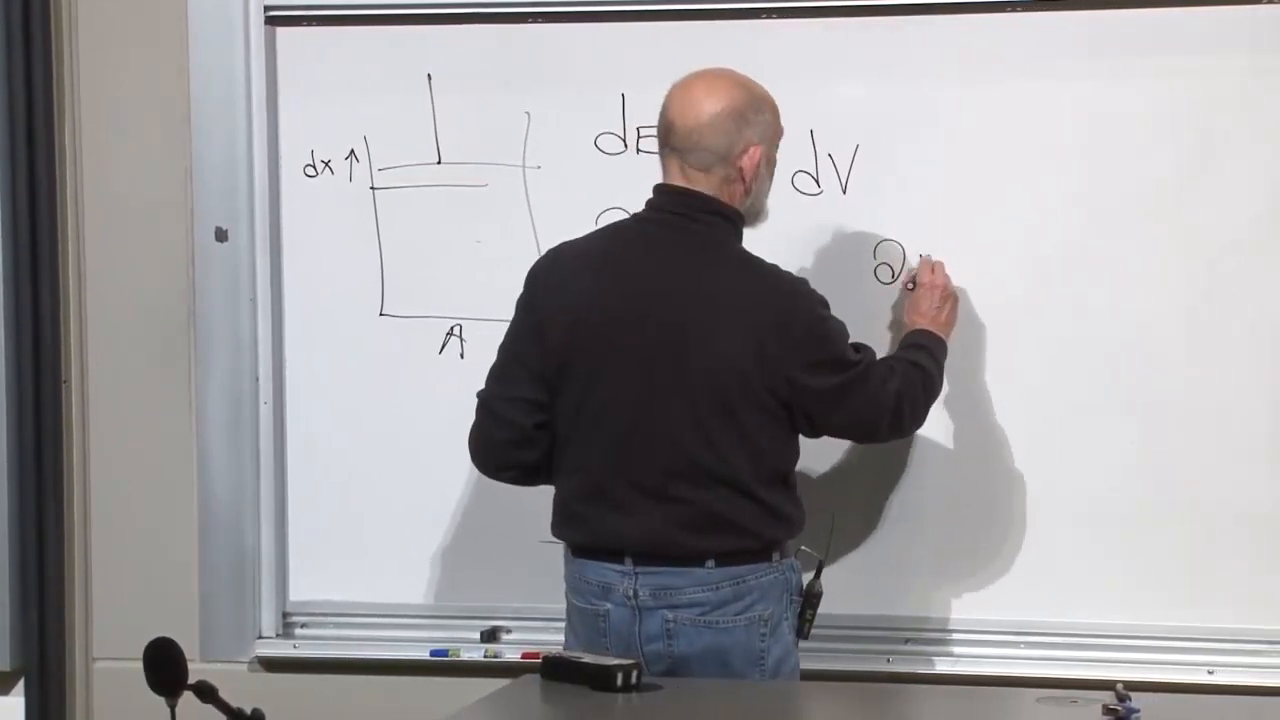
\includegraphics[width=0.90\textwidth]{lecture_05_figure_04.png}\caption{미분 보조정리를 완성하는 약분 단계에서의 일정 엔트로피 등고선 계산.}\lectureframe{00:36:10}\end{figure}

기하학적 그림은 장식이 아니다. 겉보기에는 낯선 고정 \(S\) 미분을 독립 좌표 \(T\)와 \(V\)에 대한 보통의 편미분으로 계산할 수 있는 이유를 설명해 준다. 유도 과정에서 \(\delta E/\delta V\)라고 쓰면 기호가 지정된 경로를 따라가는 작은 변화량들의 비를 나타낸다는 점을 상기하는 데 도움이 된다.

\begin{classroomqa}\audiencequestion{\(dE\)를 전개하는 것은 편미분의 통상적인 정의를 쓰는 것뿐인가요?}
\lecturerresponse{그렇습니다. 전미분에는 특별한 점이 없습니다. 추가되는 것은 나중에 \(dS=0\)인 등고선으로 제한하는 단계뿐이며, 이때 \(dT\)와 \(dV\)의 관계가 정해집니다.
\lecturetimestamp{00:29:26--00:29:32}}\end{classroomqa}

\begin{classroomqa}
\audiencequestion{상쇄가
\((\partial S/\partial T)_V\)이 0이 아니어야만 성립하나요?}
\lecturerresponse{그렇습니다. 일반적인 안정된 계에서는
\[
 \left(\frac{\partial S}{\partial T}\right)_V
 =\frac{C_V}{T}>0,
\]
따라서 나눗셈이 정당합니다. 예외적인 점에서는 별도로 주의해야 합니다. 해밀토니안이 고정된 상태에서 온도를 높이면 정준 에너지 분포가 넓어지고 엔트로피는 대개 증가하며, 온도를 낮추면 분포는 좁아집니다. 이것이 단조성 논증에서 물리적으로 올바른 방향입니다.
\lecturetimestamp{00:36:50--00:37:47}}
\end{classroomqa}

\section{피스톤이 한 일과 단열 조건}

이제 이 미분에 물리적 의미를 부여하자. 단면적이 \(\mathcal A\)인 피스톤을 생각하자. 피스톤이 바깥쪽으로 \(dx\)만큼 움직이면,
\begin{equation}
 dV=\mathcal A\,dx.
 \label{eq:sm5-piston-volume}
\end{equation}
기체는 피스톤에 \(P\mathcal A\)의 힘을 가하므로 기체가 한 일은
\begin{equation}
 \delta W_{\mathrm{by}}=P\mathcal A\,dx=P\,dV.
 \label{eq:sm5-piston-work}
\end{equation}
기체에 열이 들어오지 않으면 에너지 보존에 따라
\begin{equation}
 dE=-P\,dV.
 \label{eq:sm5-adiabatic-work}
\end{equation}
부호는 물리적 의미를 갖는다. 팽창 중에는 기체가 피스톤을 들어 올리거나 가속하고, 기체 자체의 에너지는 감소한다.

\begin{figure}[t]\centering
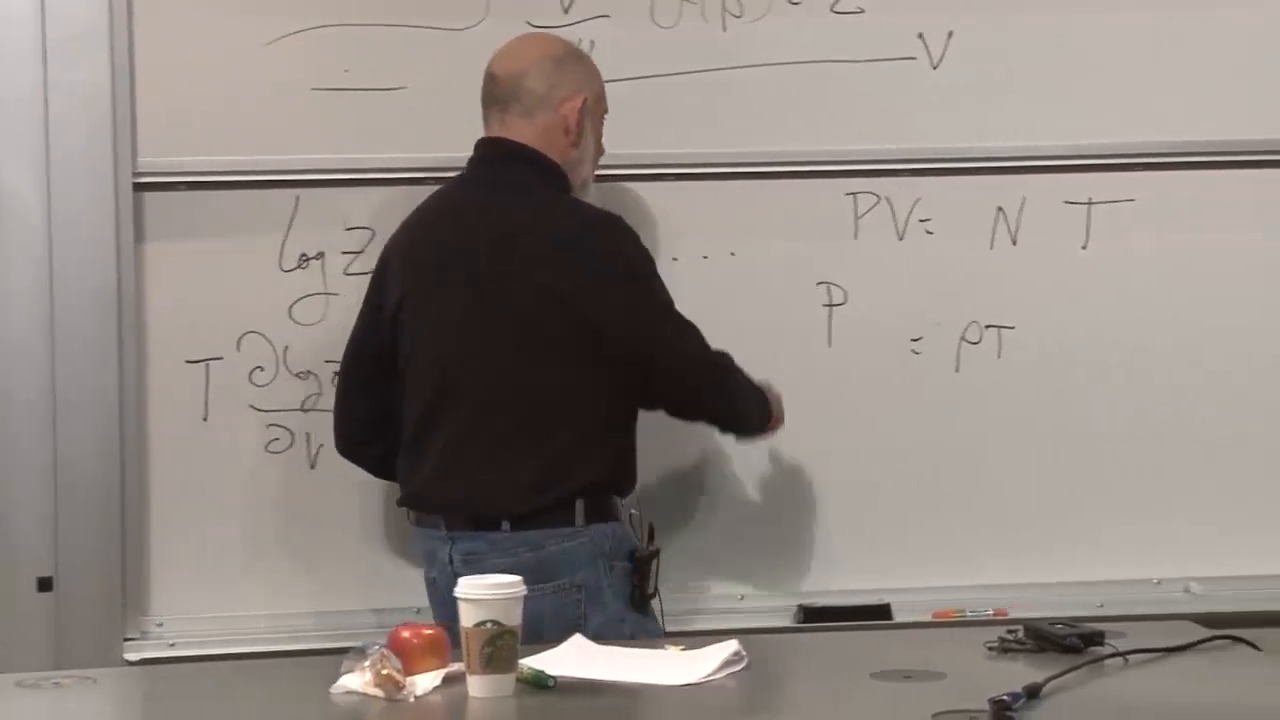
\includegraphics[width=0.90\textwidth]{lecture_05_figure_05.png}\caption{피스톤의 기하와 완성된 일의 관계 \(dE=-P\,dV\).}\lectureframe{00:43:10}\end{figure}

두 가지 조건을 반드시 만족해야 한다. 계가 평형에 임의로 가까운 상태를 유지할 만큼 피스톤이 천천히 움직여야 하고, 열이 공급되지 않도록 벽이 단열되어야 한다. 피스톤을 급히 당기면 움직이는 동안 분자가 후퇴하는 피스톤에 하나도 도달하지 못할 만큼 빠를 수 있다. 급격히 압축하면 충격파가 발생한다. 어느 과정도 평형 상태들의 연속으로 나타낼 수 없다.

\emph{단열}이라는 말은 열전달이 없다는 뜻으로 쓰이기도 하고 변화가 느리다는 뜻으로 쓰이기도 한다. 여기서 필요한 가역 과정에는 두 의미가 모두 들어간다. 변화는 준정적이며 열적으로 단열되어야 한다. 이 조건에서는 엔트로피도 일정하다.

\begin{classroomqa}\audiencequestion{단열 변화에서 엔트로피가 일정하게 유지되는 이유는 무엇인가요?}
\lecturerresponse{계를 양자역학적으로 생각해 봅시다. 다체 에너지 준위는 부피에 따라 달라집니다. \(V\)가 천천히 변하면 단열 정리에 따라 점유된 각 준위는 준위의 표지 사이에서 전이하지 않고 연속적으로 그 다음 준위로 이어집니다. 에너지 \(E_i(V)\)는 변하지만 점유 확률 \(p_i\)는 그대로 유지됩니다. \(S=-\sum_i p_i\log p_i\)는 이 확률들에 따라 정해지므로 엔트로피도 일정하게 유지됩니다. 열교환이나 비가역 운동이 있으면 이 결론은 성립하지 않습니다.
\lecturetimestamp{00:43:37--00:49:15}}\end{classroomqa}

\begin{figure}[t]\centering
\includegraphics[width=0.90\textwidth]{lecture_05_figure_06.png}\caption{점유 확률은 준위 표지를 그대로 유지하는 동안 부피에 따라 변하는 다체 에너지 준위.}\lectureframe{00:48:50}\end{figure}

이 일정 엔트로피 경로를 따라 식 \eqref{eq:sm5-adiabatic-work}을 평가하면 압력이 다음과 같이 주어진다.
\begin{equation}
 P=-\left(\frac{\partial E}{\partial V}\right)_S.
 \label{eq:sm5-pressure-fixed-entropy}
\end{equation}
이것이 압력과 부피 사이의 켤레 관계다.

\begin{classroomqa}\audiencequestion{피스톤을 빠르게 움직이면 어떻게 되나요?}
\lecturerresponse{계가 평형에서 벗어나므로 구체적인 동역학이 중요해집니다. 급격한 압축은 충격파를 일으킵니다. 이상적인 자유 팽창에서는 분자가 피스톤에 부딪히기 전에 피스톤이 후퇴할 수 있으므로 일이 이루어지지 않고, 부피가 변해도 에너지는 일정하게 유지됩니다. 이후 기체는 엔트로피가 증가한 상태로 평형에 이르도록 완화됩니다. 이런 과정은 \eqref{eq:sm5-pressure-fixed-entropy}의 단일 평형 미분으로 설명할 수 없습니다.
\lecturetimestamp{00:58:30--01:01:15}}\end{classroomqa}

\begin{classroomqa}\audiencequestion{변화가 느린지를 판별하는 정량적 조건은 무엇인가요?}
\lecturerresponse{외부 변화의 시간 척도는 관련된 내부 완화 시간보다 길어야 합니다. 기체의 경우 거시적 변화가 일어나는 동안 분자끼리 여러 차례 충돌하고 벽에도 여러 차례 부딪혀야 합니다. 정확한 시간 척도는 물질과 기하에 따라 달라지지만, 준정적 극한 자체는 일반적입니다.
\lecturetimestamp{01:02:09--01:03:20}}\end{classroomqa}

\section{단열 에너지에서 분배함수로}

물리적으로는 식 \eqref{eq:sm5-pressure-fixed-entropy}이 맞지만 계산하기 편한 형태는 아직 아니다. 정준 통계역학에서는 온도의 함수가 자연스럽게 주어진다. 볼츠만 가중치에 \(T\)가 직접 들어가기 때문이다. 미적분 보조정리를 이용하면 다루기 까다로운 고정 엔트로피 미분을 계산에 편리한 형태로 바꿀 수 있다.
\begin{align}
 P
 &=
 -\left(\frac{\partial E}{\partial V}\right)_T
 +
 \left(\frac{\partial E}{\partial S}\right)_V
 \left(\frac{\partial S}{\partial V}\right)_T.
 \label{eq:sm5-pressure-lemma-substitution}
\end{align}
부피가 고정된 상태에서 제1법칙에 따르면 \(dE=T\,dS\)이므로,
\begin{equation}
 \left(\frac{\partial E}{\partial S}\right)_V=T.
 \label{eq:sm5-e-s-temperature}
\end{equation}
따라서
\begin{equation}
 P=
 -\left(\frac{\partial E}{\partial V}\right)_T
 +
 T\left(\frac{\partial S}{\partial V}\right)_T.
 \label{eq:sm5-pressure-fixed-temperature-pieces}
\end{equation}

\begin{classroomqa}\audiencequestion{압력 공식의 마이너스 부호는 어디서 나오나요?}
\lecturerresponse{기체가 한 일에서 비롯됩니다. 단열 팽창 중에는 \(dE=-P\,dV\)입니다. 미적분 보조정리 자체에는 두 항 사이에 마이너스 부호가 있고, \(P=-(\partial E/\partial V)_S\)의 전체 마이너스 부호가 두 항의 부호를 모두 뒤집어 \eqref{eq:sm5-pressure-fixed-temperature-pieces}를 만들어 냅니다.
\lecturetimestamp{00:52:40--00:53:14}}\end{classroomqa}

두 미분 모두에서 \(T\)를 고정하므로,
\begin{align}
 P
 &=
 -\left(\frac{\partial}{\partial V}(E-TS)\right)_T \notag\\
 &=
 -\left(\frac{\partial A}{\partial V}\right)_T.
 \label{eq:sm5-pressure-free-energy}
\end{align}
마지막으로 \(A=-T\log Z\)를 대입하면,
\begin{equation}
 \boxed{
 P=
 T\left(\frac{\partial\log Z}{\partial V}\right)_T
 }.
 \label{eq:sm5-pressure-log-z}
\end{equation}

\begin{figure}[t]\centering
\includegraphics[width=0.90\textwidth]{lecture_05_figure_07.png}\caption{논증을 고정 온도에서 정리하면 다음과 같다.
\(P=-(\partial A/\partial V)_T
=T(\partial\log Z/\partial V)_T\).}\lectureframe{00:55:55}\end{figure}

식 \eqref{eq:sm5-pressure-log-z}에는 이상기체라는 가정이 전혀 들어 있지 않다. 상호작용하는 유체, 플라스마 또는 고체의 분배함수를 계산할 수 있다면 같은 미분으로 압력을 구할 수 있다. 더 일반적으로는 적절한 열역학 퍼텐셜을 미분해 모든 외부 제어변수에 대한 켤레 응답을 얻는다. 분배함수는 이러한 여러 응답을 한데 담아낸다. \(\log Z\)를 \(\beta\)에 대해 미분하면 에너지가 나오고, 부피에 대해 미분하면 압력이 나온다.

\section{이상기체 상태방정식}

이제서야 \(N\)개의 비상호작용 입자로 특수화하자. 고전적 위상공간 정규화를 유지하면,
\begin{equation}
 Z_N=
 \frac{1}{N!h^{3N}}
 \int d^{3N}q\,d^{3N}p\,
 \exp\!\left[
 -\beta\sum_{a=1}^{N}\frac{\mathbf p_a^2}{2m}
 \right].
 \label{eq:sm5-ideal-gas-partition-integral}
\end{equation}
위치 좌표가 \(3N\)개, 운동량 좌표가 \(3N\)개 있다. 해밀토니안은 위치에 의존하지 않으므로 입자마다 용기 부피에 해당하는 인수가 하나씩 생긴다.
\begin{equation}
 Z_N=
 \frac{V^N}{N!h^{3N}}I_p(\beta),
 \label{eq:sm5-ideal-gas-factorization}
\end{equation}
여기서 운동량 적분 전체인 \(I_p(\beta)\)는 \(V\)에 의존하지 않는다.

\begin{classroomqa}\audiencequestion{위치 적분은 왜 \(3N\)개이고 운동량 적분은 왜 \(3N\)개인가요?}
\lecturerresponse{입자 \(N\)개 각각에는 공간 좌표가 세 개, 그 켤레 운동량 성분이 세 개 있습니다. 위상공간의 각 절반에 있는 좌표 수는 \(3N\)개입니다. \(N\)개의 입자에 \(3N\)개의 입자를 더하는 것이 아닙니다.
\lecturetimestamp{01:04:19--01:04:28}}\end{classroomqa}

로그를 취하면 부피 의존성이 분리된다.
\begin{equation}
 \log Z_N
 =
 N\log V-\log N!-3N\log h+\log I_p(\beta).
 \label{eq:sm5-log-ideal-gas-partition}
\end{equation}
인수 \(1/N!\), \(h^{-3N}\), \(I_p(\beta)\)는 모두 부피와 무관하다. 절대 엔트로피와 다른 문제에는 중요하지만, 이 미분에는 영향을 주지 않는다. 따라서
\begin{equation}
 \left(\frac{\partial\log Z_N}{\partial V}\right)_T
 =\frac{N}{V}.
 \label{eq:sm5-log-z-volume-derivative}
\end{equation}
식 \eqref{eq:sm5-pressure-log-z}에서 곧바로 다음을 얻는다.
\begin{equation}
 P=\frac{NT}{V},
 \qquad
 \boxed{PV=NT}.
 \label{eq:sm5-ideal-gas-law}
\end{equation}

\begin{classroomqa}\audiencequestion{\(N\)는 볼츠만 분포를 유도할 때 사용한 복제계 수를 여전히 세나요?}
\lecturerresponse{아닙니다. 복제계 구성은 앞선 유도에서 계수를 세기 위한 도구였으며, 이제는 더 이상 쓰이지 않습니다. 여기서 \(N\)는 이 기체 시료 하나에 들어 있는 실제 입자 수입니다.
\lecturetimestamp{01:07:38--01:08:05}}\end{classroomqa}

수밀도를 다음과 같이 정의하면,
\begin{equation}
 \rho=\frac{N}{V}
 \label{eq:sm5-number-density}
\end{equation}
동등한 형태로 다음을 얻는다.
\begin{equation}
 P=\rho T.
 \label{eq:sm5-density-equation-of-state}
\end{equation}

\begin{classroomqa}\audiencequestion{수밀도 형태를 얻으려면 \(N\)로 나눠야 하나요, 아니면 \(V\)로 나눠야 하나요?}
\lecturerresponse{\(PV=NT\)을 \(V\)로 나누면 됩니다.
\(P=(N/V)T=\rho T\) 여기서 \(\rho\)는 질량 밀도가 아니라 수밀도입니다.
\lecturetimestamp{01:08:45--01:09:16}}\end{classroomqa}

\begin{figure}[t]\centering
\includegraphics[width=0.90\textwidth]{lecture_05_figure_08.png}\caption{\(\log Z\)의 부피 미분과 그로부터 얻는 이상기체 상태방정식 \(PV=NT\), 즉 \(P=\rho T\).}\lectureframe{01:09:25}\end{figure}

실험실 온도 \(T_K\)를 다시 쓰면,
\begin{equation}
 PV=Nk_BT_K.
 \label{eq:sm5-ideal-gas-law-laboratory}
\end{equation}
익숙한 결과가 운동론적 직관과 일치한다. 그러나 이제 그 유도는 자유 기체를 훨씬 넘어 적용되는 체계에 근거한다.

\section{두 번째 성과: 평형 요동}

압력 계산은 끝났지만, 약속한 질문 하나가 남아 있다. 분배함수에서 또 무엇을 얻을 수 있을까? 열저장고와 열접촉 중인 계를 생각해 보자. 이 계의 에너지는 고정되어 있지 않다. 에너지가 드나들기 때문에 반복해서 측정한 값은 정준 앙상블 평균을 중심으로 요동한다.

\begin{classroomqa}\audiencequestion{이제 약속했던 요동을 계산할 수 있나요?}
\lecturerresponse{그렇습니다. 남은 시간을 활용해 같은 원리를 한 번 더 보여 주겠습니다. \(Z\)의 미분에는 측정 가능한 열역학 정보가 담겨 있습니다.
\lecturetimestamp{01:10:37--01:10:50}}\end{classroomqa}

\subsection{분산과 표준편차}

\(x\)이 \(\langle x\rangle=0\)인 확률변수일 때, 분포의 폭을 나타내는 양은 \(\langle x^2\rangle\)이다. 일반적인 분포에서는 변수를 평균만큼 이동시켜 중심화한다.
\begin{equation}
 \delta x=x-\langle x\rangle.
 \label{eq:sm5-centered-variable}
\end{equation}
이 중심화된 변수의 평균은 0이며,
\begin{equation}
 \langle\delta x\rangle
 =
 \langle x\rangle-\langle x\rangle=0,
 \label{eq:sm5-centered-mean}
\end{equation}
평균제곱은 다음과 같다.
\begin{align}
 (\Delta x)^2
 &\equiv
 \left\langle\left(x-\langle x\rangle\right)^2\right\rangle \notag\\
 &=
 \langle x^2\rangle
 -2\langle x\rangle^2
 +\langle x\rangle^2 \notag\\
 &=
 \langle x^2\rangle-\langle x\rangle^2.
 \label{eq:sm5-variance}
\end{align}
이것이 분산이다. 분산의 양의 제곱근 \(\Delta x\)은 표준편차이다.

\begin{classroomqa}\audiencequestion{\(x-\langle x\rangle\)의 평균이 정확히 0인 이유는 무엇인가요?}
\lecturerresponse{평균 연산은 선형이고 \(\langle x\rangle\)는 이미 수입니다. 따라서
\(\langle x-\langle x\rangle\rangle
=\langle x\rangle-\langle x\rangle=0\)입니다.
\lecturetimestamp{01:14:02--01:14:22}}\end{classroomqa}

\begin{classroomqa}\audiencequestion{제곱 요동, 분산, 제곱평균제곱근 폭, 표준편차는 어떻게 다른가요?}
\lecturerresponse{분산은
\((\Delta x)^2=\langle x^2\rangle-\langle x\rangle^2\)입니다.
표준편차는 그 제곱근인 \(\Delta x\)입니다. 평균이 0인 변수에서는 표준편차가 제곱평균제곱근 값과도 같습니다.
\lecturetimestamp{01:16:39--01:18:38}}\end{classroomqa}

\begin{figure}[t]\centering
\includegraphics[width=0.90\textwidth]{lecture_05_figure_09.png}\caption{평균을 뺀 변수와 그 전개로 얻는 결과 \((\Delta x)^2=\langle x^2\rangle-\langle x\rangle^2\).}\lectureframe{01:17:20}\end{figure}

\subsection{분배함수에서 에너지 모멘트 구하기}

정준 앙상블에서는
\begin{align}
 \langle E\rangle
 &=
 \frac{1}{Z}\sum_i E_i e^{-\beta E_i} \notag\\
 &=
 -\frac{1}{Z}\frac{\partial Z}{\partial\beta}
 =
 -\frac{\partial\log Z}{\partial\beta}.
 \label{eq:sm5-mean-energy-from-z}
\end{align}
\(E_i\)를 인수 하나 곱하는 것은 \(\beta\)에 대한 음의 미분 한 번으로 얻는다. 두 번째 미분을 취하면 \(E_i^2\)가 나온다.
\begin{equation}
 \langle E^2\rangle
 =
 \frac{1}{Z}\sum_i E_i^2e^{-\beta E_i}
 =
 \frac{1}{Z}\frac{\partial^2 Z}{\partial\beta^2}.
 \label{eq:sm5-second-energy-moment}
\end{equation}
따라서 에너지 분산은 다음과 같다.
\begin{align}
 (\Delta E)^2
 &=
 \langle E^2\rangle-\langle E\rangle^2 \notag\\
 &=
 \frac{1}{Z}\frac{\partial^2Z}{\partial\beta^2}
 -
 \frac{1}{Z^2}
 \left(\frac{\partial Z}{\partial\beta}\right)^2 \notag\\
 &=
 \frac{\partial^2\log Z}{\partial\beta^2}
 =
 -\frac{\partial\langle E\rangle}{\partial\beta}.
 \label{eq:sm5-energy-variance-beta}
\end{align}
이번에도 복잡해 보이는 물리량이 \(\log Z\)의 미분으로 표현된다.

\begin{figure}[t]\centering
\includegraphics[width=0.90\textwidth]{lecture_05_figure_10.png}\caption{에너지 분산으로 확인되는 \(\beta\)에 대한 \(\log Z\)의 두 번째 미분.}\lectureframe{01:29:00}\end{figure}

\subsection{열용량과 요동의 크기}

강의에서 쓰는 단위에서는 \(T=1/\beta\)이므로,
\begin{equation}
 -\frac{\partial}{\partial\beta}
 =
 T^2\frac{\partial}{\partial T}.
 \label{eq:sm5-beta-temperature-derivative}
\end{equation}
부피가 고정된 상태에서 시료 전체의 열용량을 다음과 같이 정의하자.
\begin{equation}
 C_V\equiv
 \left(\frac{\partial\langle E\rangle}{\partial T}\right)_V.
 \label{eq:sm5-heat-capacity}
\end{equation}
그러면 식 \eqref{eq:sm5-energy-variance-beta}은 다음과 같이 된다.
\begin{equation}
 \boxed{(\Delta E)^2=T^2C_V}
 \qquad (k_B=1).
 \label{eq:sm5-energy-fluctuation-lecture-units}
\end{equation}
실험실 온도 \(T_K\)에서는 \(\beta=(k_BT_K)^{-1}\)이므로,
\begin{equation}
 \boxed{(\Delta E)^2=k_BT_K^2C_V}.
 \label{eq:sm5-energy-fluctuation-laboratory}
\end{equation}

\begin{figure}[t]\centering
\includegraphics[width=0.90\textwidth]{lecture_05_figure_11.png}\caption{\(\beta\) 미분을 부피 고정 열용량으로 변환하고 \(k_B\) 인수를 복원한 결과.}\lectureframe{01:31:10}\end{figure}

\begin{classroomqa}\audiencequestion{미분에서 부피를 고정할지 압력을 고정할지 명시해야 하나요?}
\lecturerresponse{그렇습니다. 이 정준 유도에서는 \(V\)를 포함해 해밀토니안의 외부 제어변수를 고정합니다. 따라서 얻는 물리량은 \(C_V\)입니다. 정압 앙상블에서는 부피와 일이 요동하므로 그에 맞는 열역학 퍼텐셜이 필요합니다. 식 \eqref{eq:sm5-energy-fluctuation-laboratory}에서 \(C_V\)를 \(C_P\)로 단순히 바꿔 쓸 수는 없습니다.
\lecturetimestamp{01:29:01--01:29:28; 01:32:50--01:33:21}}\end{classroomqa}

\begin{classroomqa}\audiencequestion{\(C_V\)는 물질 상수인가요?}
\lecturerresponse{일반적으로 그렇지 않습니다. 온도, 부피, 상, 조성에 따라 달라질 수 있습니다. 또한 여기서 \(C_V\)는 시료 전체의 열용량이므로 크기에 비례하는 양입니다. 비열을 구하려면 질량, 입자 수 또는 물질량으로 나누어야 합니다.
\lecturetimestamp{01:31:47--01:32:21; 01:33:23--01:34:55}}\end{classroomqa}

보통의 크기에 비례하는 물질에서는 \(C_V\)가 \(N\)에 비례하므로 \((\Delta E)^2\)도 \(N\)에 비례하고 \(\Delta E\)는 \(\sqrt{N}\)에 비례한다. 평균 에너지 자체는 \(N\)에 비례한다. 따라서
\begin{equation}
 \frac{\Delta E}{\langle E\rangle}\sim\frac{1}{\sqrt{N}}.
 \label{eq:sm5-relative-fluctuation-scaling}
\end{equation}
거시적 계에서는 상대 요동이 매우 작지만 미시적 시료에서는 직접 관측된다. 식 \eqref{eq:sm5-energy-fluctuation-laboratory}에 \(k_B\)가 등장한다는 것은 열역학적 물리량과 분자의 이산성 사이의 연결을 나타낸다. 다시 말해 거시적 단위와 아보가드로 수 규모의 계수를 연결한다.

압력과 요동은 이제 같은 대상에서 나왔다.
\[
 P=T\left(\frac{\partial\log Z}{\partial V}\right)_T,
 \qquad
 (\Delta E)^2=\frac{\partial^2\log Z}{\partial\beta^2}.
\]
이것이 핵심 교훈이다. 올바른 제약 조건을 찾아내면 분배함수는 확률을 정규화하는 데 그치지 않는다. 그 미분들이 계에서 측정 가능한 열역학적 성질을 체계적으로 정리해 준다.